Decomposition is a mathematical technique to convert a large-base number into a mathematical formula expressing the same value in a smaller base. This section will explain number decomposition and polynomial decomposition. 

\subsection{Number Decomposition}
\label{subsec:number-decomp}
Suppose we have the number $\gamma$ modulo $q$. Number decomposition expresses $\gamma$ as a sum of multiple numbers in base $\beta$ as follows: 

$ $

$\gamma = \gamma_1 \dfrac{q}{\beta^1} + \gamma_2 \dfrac{q}{\beta^2} + \cdots + \gamma_l \dfrac{q}{\beta^l}  $

$ $

\noindent , where each of the $\gamma_i$ term represents a base-$\beta$ value shifted $i$ bits (which is a multiple of $\text{log}_2 \beta$) to the left. We call $l$ the level of decomposition. This is visually shown in \autoref{fig:decomp}. %We will cover the GLev ciphertext formula in \autoref{sec:glev}.

\begin{figure}[h!]
    \centering
  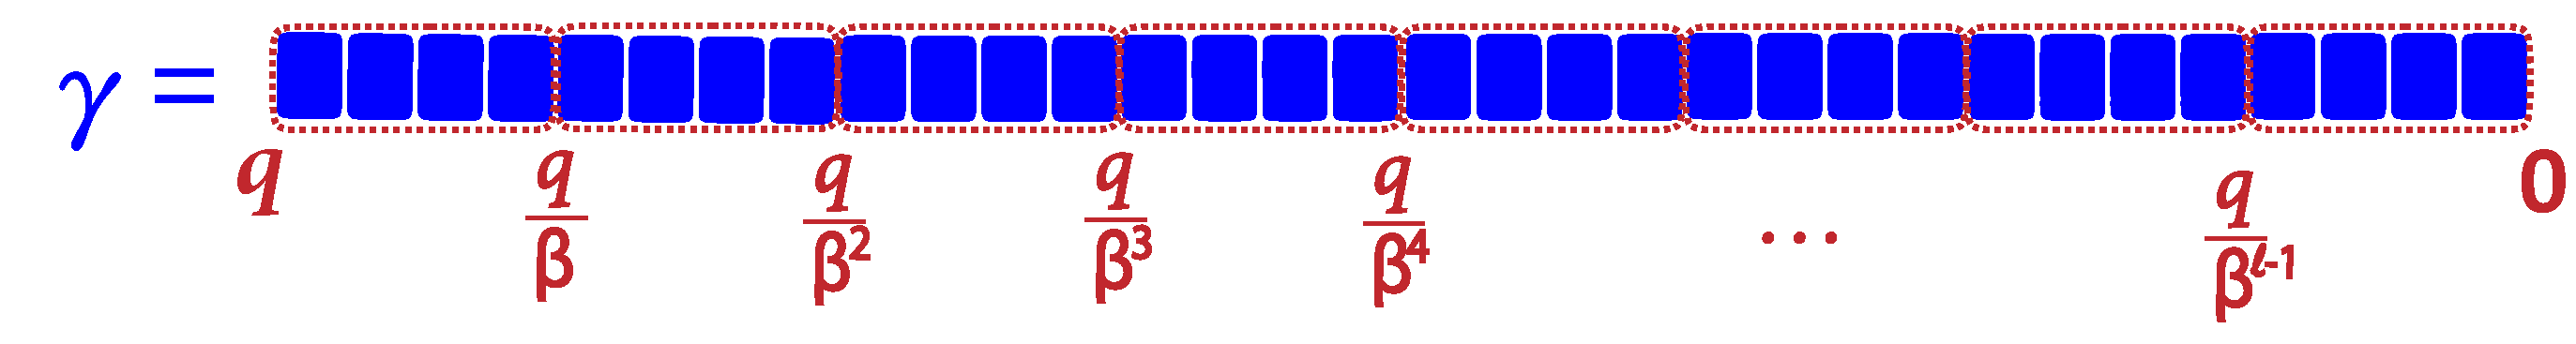
\includegraphics[width=0.8\linewidth]{figures/decomp.pdf}
  \caption{An illustration of number decomposition.}
  \label{fig:decomp}
\end{figure}

We define the decomposition of number $\gamma$ into base $\beta$ with level $l$ as follows:


$ $

$\textsf{Decomp}^{\beta, l}(\gamma) = (\gamma_1, \gamma_2, \text{ } \cdots , \text{ } \gamma_l)$.
 
$ $

Number decomposition is also called radix decomposition, where the base $\beta$ is called a radix. 


\subsubsection{Example}

Suppose we have the number $\gamma = 13 \bmod q$, where $q = 16$. Suppose we want to decompose 13 with the base $\beta = 2$ and level $l = 4$. Then, 13 is decomposed as follows:

$ $

$13 = 1 \cdot \dfrac{16}{2^1} + 1 \cdot \dfrac{16}{2^2} + 0 \cdot \dfrac{16}{2^3} + 1 \cdot \dfrac{16}{2^4}$

$ $

$\textsf{Decomp}^{2, 4}(13) = (1, 1, 0, 1)$


\subsection{Polynomial Decomposition}
\label{subsec:poly-decomp}

This time, suppose we have polynomial $f$ in the polynomial ring $\bm{\mathbb{Z}_q[x] / (x^n + 1)}$. Therefore, each coefficient $c_i$ of $f$ is an integer modulo $q$. Polynomial decomposition expresses $f$ as a sum of multiple polynomials in base $\beta$ and level $l$ as follows:


\begin{tcolorbox}[title={\textbf{\tboxlabel{\ref*{subsec:poly-decomp}} Polynomial Decomposition}}]

Given $f \in \mathbb{Z}_q[z]/(x^n+1)$, where:

$ $

$f = f_1 \dfrac{q}{\beta^1} + f _2\dfrac{q}{\beta^2} + \cdots + f_l \dfrac{q}{\beta^l}  $

$ $

We denote the decomposition of polynomial $f$ into base $\beta$ with level $l$ as follows:

$ $

$\textsf{Decomp}^{\beta, l}(f) = (f_1, f_2, \text{ } \cdots , \text{ } f_l)$
 $ $
\end{tcolorbox}




\subsubsection{Example}

Suppose we have the following polynomial in the polynomial ring $\mathbb{Z}_{16}[x] / (x^4 + 1)$:

$ $

$f = 6x^3 + 3x^2 + 14x + 7 \in \mathbb{Z}_{16}[x] / (x^4 + 1)$

$ $

Suppose we want to decompose the above polynomial with base $\beta = 4$ and level $l = 2$. Then, each degree's coefficient of the polynomial $f$ is decomposed as follows:

$ $

$\bm{x^3}$: $6 = \color{blue}{1 \cdot \dfrac{16}{4^1}} \color{black}+ \color{red}{2 \cdot \dfrac{16}{4^2}}$

$\bm{x^2}$: $3 = \color{blue}{0 \cdot \dfrac{16}{4^1}} \color{black}+ \color{red}{3 \cdot \dfrac{16}{4^2}}$

$\bm{x^1}$: $14 = \color{blue}{3 \cdot \dfrac{16}{4^1}} \color{black}+ \color{red}{2 \cdot \dfrac{16}{4^2}}$

$\bm{x^0}$: $7 = \color{blue}{1 \cdot \dfrac{16}{4^1}} \color{black}+ \color{red}{3 \cdot \dfrac{16}{4^2}}$

$ $

The decomposed polynomial is as follows:

$f = 6x^3 + 3x^2 + 14x + 7 = \color{blue}{(1x^3 + 0x^2 + 3x + 1) \cdot \dfrac{16}{4^1}} \color{black}+ \color{red}{(2x^3 + 3x^2 + 2x + 3) \cdot \dfrac{16}{4^2}} \color{black}$

$ $

$\textsf{Decomp}^{4, 2}(6x^3 + 3x^2 + 14x + 7) = (1x^3 + 0x^2 + 3x + 1, 2x^3 + 3x^2 + 2x + 3)$

\subsubsection{Discussion}

Note that after decomposition, the original coefficients of the polynomial got reduced to smaller numbers. This characteristic is importantly used in homomorphic encryption's multiplication, for reducing the growth rate of the noise. Normally, the polynomial coefficients of ciphertexts are large because they are uniformly random numbers. Reducing such big constants is important to reduce the noise growth during homomorphic multiplication. We will discuss this more in detail in \autoref{subsec:tfhe-mult-cipher}.


\subsection{Approximate Decomposition}
\label{subsec:approx-decomp}

\begin{figure}[h!]
    \centering
  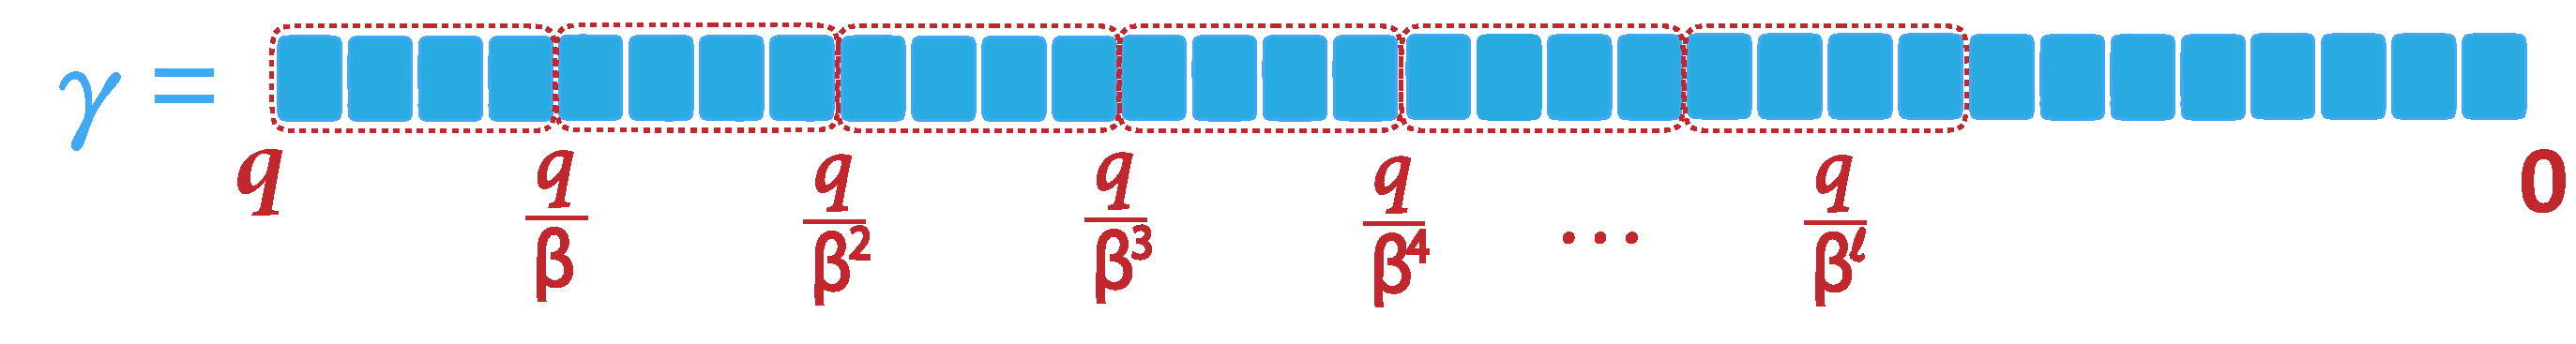
\includegraphics[width=0.7\linewidth]{figures/decomp3.pdf}
  \caption{An illustration of approximate decomposition}
  \label{fig:decomp3}
\end{figure}

If the base $\beta$ does not divide the modulo $q$, then there exists no level $l$ such that $\beta^l \text{ } | \text{ } q$, thus some lower bits of $q$ have to be drawn away during decomposition, as shown in \autoref{fig:decomp3}. Such lower bits can be rounded to the nearest multiple of $\dfrac{q}{\beta^l}$ during decomposition. In such a case, the decomposition is an approximate decomposition. 




\subsection{Gadget Decomposition}
\label{subsec:gadget-decomposition}

Gadget decomposition is a generalized form of number decomposition (\autoref{subsec:number-decomp}). In number decomposition, a number $\gamma$ is decomposed as follows: 

$\gamma = \gamma_1 \dfrac{q}{\beta^1} + \gamma_2 \dfrac{q}{\beta^2} + \cdots + \gamma_l \dfrac{q}{\beta^l} $

$ $

In gadget decomposition, we decompose $\gamma$ as follows: 

$\gamma = \gamma_1 g_1 + \gamma_2 g_2 + \cdots + \gamma_l g_l $

$ $

We denote $\vec{g} = (g_1, g_2, \cdots, g_l)$ as a gadget vector, and $\textsf{Decomp}^{\vec{g}}(\gamma) = (\gamma_1, \gamma_2, \text{ } \cdots , \text{ } \gamma_l) $

$ $

Then, $\gamma = \langle \textsf{Decomp}^{\vec{g}}(\gamma), \vec{g} \rangle $

$ $

In the case of number decomposition (\autoref{subsec:number-decomp}), its gadget vector is $\vec{g} = \Bigg(\dfrac{q}{\beta}, \dfrac{q}{\beta^2}, \cdots, \dfrac{q}{\beta^l}\Bigg)$.

%After ciphertext-to-plaintext multiplication $\Lambda \cdot \textsf{GLWE}_{S, \sigma}(M)$, the noise grows from $E$ to $E' = \Lambda \cdot E$. To limit this noise growth, we introduce a technique called gadget decomposition, which consists of decomposed (\autoref{subsec:number-decomp}) $\Lambda$ and an GLev encryption (\autoref{subsec:glev-enc}) of $M$ as follows:

%$\Lambda = \Lambda_1 \dfrac{q}{\beta^1} + \Lambda_2 \dfrac{q}{\beta^2} + \cdots + \Lambda_l \dfrac{q}{\beta^l} \longrightarrow \textsf{Decomp}^{\beta, l}(\Lambda) = (\Lambda_1, \Lambda_2, \cdots, \Lambda_l)$

%$ $

%$\textsf{GLev}_{S, \sigma}^{\beta, l}(\Delta M) = \Bigg\{ \textsf{GLWE}_{S, \sigma}\left(\Delta M \dfrac{q}{\beta^1}\right), \textsf{GLWE}_{S, \sigma}\left(\Delta M \dfrac{q}{\beta^2}\right), \cdots \textsf{GLWE}_{S, \sigma}\left(\Delta M \dfrac{q}{\beta^l}\right) \Bigg\}$

%$ $

%Based on decomposed $\Lambda$ and the GLev encryption of $M$, we can compute the ciphertext-to-plaintext multiplication of $M \cdot \Lambda$ as follows:

%$\langle \textsf{Decomp}^{\beta, l}(\Lambda), \textsf{GLev}_{S, \sigma}^{\beta, l}(\Delta M) \rangle$


%$= \Lambda_1 \cdot \textsf{GLWE}_{S, \sigma}\left(\Delta M \dfrac{q}{\beta^1}\right) +  \Lambda_2 \cdot \textsf{GLWE}_{S, \sigma}\left(\Delta M \dfrac{q}{\beta^2}\right) \cdots \Lambda_l \cdot \textsf{GLWE}_{S, \sigma}\left(\Delta M \dfrac{q}{\beta^l}\right)$

%$= \textsf{GLWE}_{S, \sigma}\left(\Delta M \cdot \Lambda_1\dfrac{q}{\beta^1}\right) + \textsf{GLWE}_{S, \sigma}\left(\Delta M  \cdot \Lambda_2\dfrac{q}{\beta^2}\right) \cdots \cdot \textsf{GLWE}_{S, \sigma}\left(\Delta M  \cdot \Lambda_l\dfrac{q}{\beta^l}\right)$

%$= \textsf{GLWE}_{S, \sigma}\left(\Delta M  \cdot \left(  \Lambda_1 \dfrac{q}{\beta^1} + \Lambda_2 \dfrac{q}{\beta^2} + \cdots + \Lambda_l \dfrac{q}{\beta^l} \right) \right)$

%$= \textsf{GLWE}_{S, \sigma}(\Delta (M \cdot \Lambda))$

%$ $

%Given the noise of each GLWE ciphertext in the GLev ciphertext above is $E_i$, the aggregate noise of the final ciphertext-to-plaintext multiplication is $\sum\limits_{i=0}^{l}E_i$, which is much smaller than the original noise $\Lambda \cdot e$ in \tboxlabel{\ref*{subsec:tfhe-mult-plain}.3}-- as $l$ is usually much smaller than $\Lambda$. This way, we can limit the noise growth of ciphertext-to-plaintext multiplication. 

%We can do gadget decomposition for any number of consecutive ciphertext-to-plaintext multiplication operations, by postponing the summation of GLWE ciphertexts to the end. However, gadget decomposition gets terminated if there is any interruption of a different operation, such as ciphertext-to-plaintext addition, ciphertext-to-ciphertext addition, or ciphertext-to-ciphertext multiplication, because in that case, the consistent format of the $GLev$ ciphertext breaks. 

%There is a more general and powerful solution to re-initialize the accumulated noise $E$ without decrypting the ciphertext, which is called bootstrapping. We will later explain the TFHE scheme's bootstrapping in \autoref{subsec:tfhe-bootstrapping}). 
